%%%%%%%%%%%%%%%%%%%%%%%%%%%%%%%%%%%%
% Slide options
%%%%%%%%%%%%%%%%%%%%%%%%%%%%%%%%%%%%

% Option 1: Slides with solutions

\documentclass[slidestop,compress,mathserif]{beamer}
\newcommand{\soln}[1]{\textit{#1}}
\newcommand{\solnGr}[1]{#1}
\usepackage{booktabs}

% Option 2: Handouts without solutions

%\documentclass[11pt,containsverbatim,handout]{beamer}
%\usepackage{pgfpages}
%\pgfpagesuselayout{4 on 1}[letterpaper,landscape,border shrink=5mm]
%\newcommand{\soln}[1]{ }
%\newcommand{\solnGr}{ }

\def\argmax{\operatornamewithlimits{arg\,max}}
\def\argmin{\operatornamewithlimits{arg\,min}}

%%%%%%%%%%%%%%%%%%%%%%%%%%%%%%%%%%%%
% Style
%%%%%%%%%%%%%%%%%%%%%%%%%%%%%%%%%%%%
%%%%%%%%%%%%%%%%%%%%%%%%%%%%%%%%%%%%%%%%%%%%%%%%%%%%%%%%%%%%%%%%%%%%%%%%
% MA213/214 shared slide style
%
% "Calm & Cool" palette + content-type callout boxes.
% Overhauled (2026) from the original OpenIntro/metropolis style:
%   - all OpenIntro visual branding removed (logo, grid, colors)
%   - a low-key cool palette (see colors below)
%   - tcolorbox callout boxes so students recognize content types
% See common/README.md for the command cheat-sheet.
%%%%%%%%%%%%%%%%%%%%%%%%%%%%%%%%%%%%%%%%%%%%%%%%%%%%%%%%%%%%%%%%%%%%%%%%

\usetheme{metropolis}

%%%%%%%%%%%%%%%%
% Packages
%%%%%%%%%%%%%%%%

\usepackage{geometry}
\usepackage{graphicx}
\usepackage{amssymb}
\usepackage{epstopdf}
\usepackage{amsmath}  	% this permits text in eqnarray among other benefits
\usepackage{url}		% produces hyperlinks
\usepackage{hyperref}	% allows for color usage in tables
\usepackage[english]{babel}
\usepackage[latin1]{inputenc}
\usepackage{colortbl}	% allows for color usage in tables
\usepackage{multirow}	% allows for rows that span multiple rows in tables
\usepackage{color}		% this package has a variety of color options
\usepackage{pgf}
\usepackage{calc}
\usepackage{ulem}
\usepackage{multicol}
\usepackage{textcomp}
\usepackage{txfonts}
\usepackage{listings}
\usepackage{tikz}
\usepackage{array}
\usepackage{wasysym}
\usepackage{fancyvrb}
\usepackage{etoolbox}             % \ifstrempty for optional box subtitles
\usepackage[most]{tcolorbox}      % content-type callout boxes
\tcbuselibrary{listings}          % R-code block (\begin{rblock})
\usepackage{fontawesome5}         % box icons

%%%%%%%%%%%%%%%%
% Remove navigation symbols
%%%%%%%%%%%%%%%%

\setbeamertemplate{navigation symbols}{}

%%%%%%%%%%%%%%%%
% "Calm & Cool" palette
%%%%%%%%%%%%%%%%

% chrome / structure / body
\definecolor{ccSlate}{HTML}{2E3742}   % frametitle bar, structure, section pages (deep neutral slate)
\definecolor{ccInk}{HTML}{2B2B2B}     % body text
\definecolor{ccWash}{HTML}{FCF8F1}    % gentle warm title-slide background wash (complements the cool blues)

% example (blue)
\definecolor{ccBlue}{HTML}{2F6690}
\definecolor{ccBlueBg}{HTML}{EAF1F7}
% interactive activity / discussion (green)
\definecolor{ccGreen}{HTML}{4E8A6B}
\definecolor{ccGreenBg}{HTML}{E9F3EC}
% solution (purple)
\definecolor{ccPurple}{HTML}{6F5499}
\definecolor{ccPurpleBg}{HTML}{EFEAF6}
% worksheet / focused work (terracotta)
\definecolor{ccTerra}{HTML}{C2693E}
\definecolor{ccTerraBg}{HTML}{FAEDE4}
% formula / definition (neutral slate)
\definecolor{ccGray}{HTML}{5C6B7A}
\definecolor{ccGrayBg}{HTML}{EEF1F4}
% caution / common pitfall (brick red)
\definecolor{ccRed}{HTML}{B23A48}
\definecolor{ccRedBg}{HTML}{FAEAEC}
% key idea / takeaway (muted gold)
\definecolor{ccGold}{HTML}{9C7A28}
\definecolor{ccGoldBg}{HTML}{F7F1DF}
% learning goals / lesson outcomes (teal)
\definecolor{ccTeal}{HTML}{2C6E6B}
\definecolor{ccTealBg}{HTML}{E6F0EF}
% learning objectives (indigo)
\definecolor{ccIndigo}{HTML}{45507A}
\definecolor{ccIndigoBg}{HTML}{ECEEF4}
% R code / output (gray)
\definecolor{ccCode}{HTML}{5F5E5A}
\definecolor{ccCodeBg}{HTML}{F4F5F6}

% neutral grays kept from the original style
\definecolor{gray}{rgb}{0.5, 0.5, 0.5}
\definecolor{darkGray}{rgb}{0.3, 0.3, 0.3}
\definecolor{darkerGray}{rgb}{0.2, 0.2, 0.2}

% Backwards-compatible aliases: old OpenIntro color names now point at the
% new palette, so existing \textcolor{oiB}{...}, \hl{...}, etc. keep working.
\colorlet{oiB}{ccBlue}
\colorlet{oiG}{ccGreen}
\colorlet{hlblue}{ccBlue}
\colorlet{rubineRed}{ccRed}
\colorlet{irishGreen}{ccGreen}
\colorlet{lightGreen}{ccGreen}

%%%%%%%%%%%%%%%%
% Restyle metropolis with the Calm & Cool chrome
%%%%%%%%%%%%%%%%

\metroset{block=fill}

\setbeamercolor{normal text}{fg=ccInk, bg=white}
\setbeamercolor{structure}{fg=ccSlate}
\setbeamercolor{alerted text}{fg=ccBlue}
\setbeamercolor{example text}{fg=ccGreen}
\setbeamercolor{frametitle}{bg=ccSlate, fg=white}
\setbeamercolor{progress bar}{fg=ccBlue}
\setbeamercolor{title separator}{fg=ccBlue}
\setbeamercolor{title}{fg=ccSlate}
\setbeamercolor{subtitle}{fg=ccBlue}
\setbeamercolor{author}{fg=ccInk}
\setbeamercolor{institute}{fg=ccGray}
\setbeamercolor{date}{fg=ccGray}
\setbeamercolor{section title}{fg=ccSlate}
\setbeamercolor{standout}{fg=white, bg=ccSlate}

% Section pages sit on the same warm wash as the title slide. We keep
% metropolis's section-title styling and just paint a full-page ccWash
% background behind it (needs >=2 pdflatex passes for the current-page node).
\setbeamertemplate{section page}{%
  \begin{tikzpicture}[remember picture, overlay]
    \fill[ccWash] (current page.south west) rectangle (current page.north east);
  \end{tikzpicture}%
  \centering
  \begin{minipage}{22em}
    \raggedright
    \usebeamercolor[fg]{section title}%
    \usebeamerfont{section title}%
    \insertsectionhead\\[-1ex]
    \usebeamertemplate*{progress bar in section page}%
    \par
  \end{minipage}\par
  \vspace{\baselineskip}
}

%%%%%%%%%%%%%%%%
% Custom inline text commands (recolored to the palette)
%%%%%%%%%%%%%%%%

% degree
\newcommand{\degree}{\ensuremath{^\circ}}

% cite
\newcommand{\ct}[1]{
\vfill
{\tiny #1}}

\newcommand{\NamedNote}[2]{
\rule{2.5cm}{0.25pt} \\ \textit{\footnotesize{\textcolor{rubineRed}{#1:} \textcolor{darkerGray}{#2}}}}

% Note
\newcommand{\Note}[1]{
\rule{2.5cm}{0.25pt} \\ \textit{\footnotesize{\textcolor{rubineRed}{Note:} \textcolor{darkerGray}{#1}}}}

% Remember
\newcommand{\Remember}[1]{\textit{\scriptsize{\textcolor{ccTerra}{Remember:} #1}}}

% expected counts
\newcommand{\ex}[1]{\textit{\textcolor{ccBlue}{#1}}}

% red
\newcommand{\red}[1]{\textit{\textcolor{rubineRed}{#1}}}

% pink
\newcommand{\pink}[1]{\textit{\textcolor{rubineRed!90!white!50}{#1}}}

% green
\newcommand{\green}[1]{\textit{\textcolor{irishGreen}{#1}}}

% orange
\newcommand{\orange}[1]{\textit{\textcolor{ccTerra}{#1}}}

% links: webURL, webLink, appLink
\newcommand{\webURL}[1]{\urlstyle{same}{ \textit{\textcolor{darkGray}{\url{#1}}}}}
\newcommand{\webLink}[2]{\href{#1}{\textcolor{darkGray}{{#2}}}}
\newcommand{\appLink}[2]{\href{#1}{\textcolor{white}{{#2}}}}

% mail
\newcommand{\mail}[1]{\href{mailto:#1}{\textit{\textcolor{darkGray}{#1}}}}

% highlighting: hl, hlGr, mathhl
\newcommand{\hl}[1]{\textit{\textcolor{hlblue}{#1}}}
\newcommand{\hlGr}[1]{\textit{\textcolor{lightGreen}{#1}}}
\newcommand{\mathhl}[1]{\textcolor{hlblue}{\ensuremath{#1}}}

%%%%%%%%%%%%%%%%
% Structural helpers (unchanged from the original)
%%%%%%%%%%%%%%%%

% two col: two columns
\newenvironment{twocol}[4]{
\begin{columns}[c]
\column{#1\textwidth}
#3
\column{#2\textwidth}
#4
\end{columns}
}

% slot (for probability calculations)
\newenvironment{slot}[2]{
\begin{array}{c}
\underline{#1} \\
#2
\end{array}
}

% pr: left and right parentheses
\newcommand{\pr}[1]{
\left( #1 \right)
}

% cancel
\newcommand{\cancel}[1]{%
    \tikz[baseline=(tocancel.base)]{
        \node[inner sep=0pt,outer sep=0pt] (tocancel) {#1};
        \draw[red, line width=0.5mm] (tocancel.south west) -- (tocancel.north east);
    }%
}

% removepagenumbers
\newcommand{\removepagenumbers}{%
  \setbeamertemplate{footline}{}
}

% change margin
\newenvironment{changemargin}[2]{%
\begin{list}{}{%
\setlength{\topsep}{0pt}%
\setlength{\leftmargin}{#1}%
\setlength{\rightmargin}{#2}%
\setlength{\listparindent}{\parindent}%
\setlength{\itemindent}{\parindent}%
\setlength{\parsep}{\parskip}%
}%
\item}{\end{list}}

% footnote
\long\def\symbolfootnote[#1]#2{\begingroup%
\def\thefootnote{\fnsymbol{footnote}}\footnote[#1]{#2}\endgroup}

% commands from the book
\newenvironment{data}[1]{\texttt{#1}}{}
\newenvironment{var}[1]{\texttt{#1}}{}
\newenvironment{resp}[1]{\texttt{#1}}{}

%%%%%%%%%%%%%%%%
% Content-type callout boxes (tcolorbox)
%
% Each type has a colored title strip (icon + label) over a light fill.
% Color = content type; the label + icon reinforce it (so the cue does
% not rely on color alone).
%%%%%%%%%%%%%%%%

\tcbset{
  cccallout/.style 2 args={
    enhanced, breakable=false,
    colback=#2, colframe=#1, colbacktitle=#1, coltitle=white,
    fonttitle=\bfseries\footnotesize,
    boxrule=0.6pt, arc=2.5pt, outer arc=2.5pt,
    left=5pt, right=5pt, top=3pt, bottom=3pt, boxsep=2pt,
    toptitle=2pt, bottomtitle=2pt, lefttitle=5pt,
    before skip=5pt, after skip=5pt,
  },
}

% One-off / collection of examples (blue): \workedexample[subtitle]{body}.
% (Named \workedexample, not \example, because beamer defines \example.)
\newtcolorbox{examplebox}[1][]{cccallout={ccBlue}{ccBlueBg},
  title={\faIcon{lightbulb}~~Example\ifstrempty{#1}{}{ \textmd{---}\ #1}}}
\newcommand{\workedexample}[2][]{\begin{examplebox}[#1]#2\end{examplebox}}

% Running-example header (blue): \examplehead{name} at the top of each frame of a
% multi-slide running example. A one-off or a collection of examples uses the
% \workedexample box above instead.
\newcommand{\examplehead}[1]{%
  \vspace{-0.4em}\par\noindent\tcbox[on line, colback=ccBlue, colframe=ccBlue, coltext=white,
    boxrule=0pt, arc=2pt, left=5pt, right=5pt, top=1pt, bottom=1pt,
    box align=base, nobeforeafter]{\footnotesize\bfseries\faIcon{lightbulb}\,Running example}%
  \ifstrempty{#1}{}{\enspace{\footnotesize\bfseries\textcolor{ccBlue}{#1}}}%
  \par\nobreak\vspace{-0.6em}{\color{ccBlue}\rule{\linewidth}{0.7pt}}\par\nobreak\vspace{-0.8em}}

% Interactive activity (green): \activity[subtitle]{body}
\newtcolorbox{activitybox}[1][]{cccallout={ccGreen}{ccGreenBg},
  title={\faIcon{users}~~Activity\ifstrempty{#1}{}{ #1}}}
\newcommand{\activity}[2][]{\begin{activitybox}[#1]#2\end{activitybox}}

% Discussion question (green): \dq{body}
\newtcolorbox{dqbox}{cccallout={ccGreen}{ccGreenBg}, title={\faIcon{comments}~~Discussion}}
\newcommand{\dq}[1]{\begin{dqbox}#1\end{dqbox}}

% Solution (purple): \solnbox{body}. Gated by the per-deck \soln toggle, so it
% shows in the instructor build and vanishes from the student handout build.
% (Named \solnbox, not \solution, because beamer already defines \solution.)
\newtcolorbox{solutionbox}{cccallout={ccPurple}{ccPurpleBg}, title={\faIcon{key}~~Solution}}
\newcommand{\solnbox}[1]{\soln{\begin{solutionbox}#1\end{solutionbox}}}

% Worksheet / focused work (terracotta): \worksheet[subtitle]{body}
\newtcolorbox{worksheetbox}[1][]{cccallout={ccTerra}{ccTerraBg},
  title={\faIcon{pencil-alt}~~Worksheet\ifstrempty{#1}{}{ #1}}}
\newcommand{\worksheet}[2][]{\begin{worksheetbox}[#1]#2\end{worksheetbox}}

% Formula / definition (neutral slate). Supports both real usages found in the
% decks: \formula{title}{body} and the bare \formula{body} (title defaults to
% "Formula"). The second group is an optional brace argument.
\newtcolorbox{formulabox}[1][Formula]{cccallout={ccGray}{ccGrayBg},
  title={\faIcon{square-root-alt}~~#1}}
\NewDocumentCommand{\formula}{m g}{%
  \IfNoValueTF{#2}%
    {\begin{formulabox}#1\end{formulabox}}%
    {\begin{formulabox}[#1]#2\end{formulabox}}}

% Common pitfall / caution (brick red): \caution[subtitle]{body}
\newtcolorbox{cautionbox}[1][]{cccallout={ccRed}{ccRedBg},
  title={\faIcon{exclamation-triangle}~~Caution\ifstrempty{#1}{}{ #1}}}
\newcommand{\caution}[2][]{\begin{cautionbox}[#1]#2\end{cautionbox}}

% Key idea / takeaway (muted gold): \keyidea[subtitle]{body}
\newtcolorbox{keyideabox}[1][]{cccallout={ccGold}{ccGoldBg},
  title={\faIcon{star}~~Key idea\ifstrempty{#1}{}{ #1}}}
\newcommand{\keyidea}[2][]{\begin{keyideabox}[#1]#2\end{keyideabox}}

% Learning goals / lesson outcomes (teal): \goals{body}. Sits under the short
% LO headings on the objectives slide; body is the "you should be able to" list.
\newtcolorbox{goalsbox}{cccallout={ccTeal}{ccTealBg}, fontupper=\footnotesize,
  top=1pt, bottom=2pt, boxsep=1pt, before skip=3pt,
  title={\faIcon{bullseye}~~By the end of today, you should be able to\ldots}}
\newcommand{\goals}[1]{\begin{goalsbox}#1\end{goalsbox}}

% Learning objectives (indigo): \objectives{body} -- the formal LO headings,
% shown alongside \goals on the objectives slide.
\newtcolorbox{objectivesbox}{cccallout={ccIndigo}{ccIndigoBg}, fontupper=\small,
  top=1pt, bottom=2pt, boxsep=1pt, before skip=3pt,
  title={\faIcon{clipboard-list}~~Learning objectives}}
\newcommand{\objectives}[1]{\begin{objectivesbox}#1\end{objectivesbox}}

% Defaults for a bare \begin{lstlisting}. Without these it inherits the listings
% package defaults: 11pt type, fixed-width columns (which spaces code out as
% "a g e _ f i t"), and no line breaking, so a long line silently runs off the
% right edge of the slide. A deck that passes its own basicstyle still wins.
% Layout only -- syntax coloring is left to the \begin{rblock} environment.
\lstset{
  basicstyle=\ttfamily\footnotesize, columns=fullflexible,
  breaklines=true, breakindent=1.5em, showstringspaces=false,
  numbers=none, frame=none}

% R code / output (gray): \begin{rblock}[subtitle] ... \end{rblock}
% NOTE: a frame containing an rblock must be declared \begin{frame}[fragile].
\lstdefinestyle{ccR}{
  language=R, basicstyle=\ttfamily\footnotesize, columns=fullflexible,
  breaklines=true, showstringspaces=false, numbers=none, frame=none,
  keywordstyle=\color{ccBlue}, commentstyle=\color{ccGreen!75!black},
  stringstyle=\color{ccTerra}}
\newtcblisting{rblock}[1][]{cccallout={ccCode}{ccCodeBg},
  title={\faIcon{terminal}~~R\ifstrempty{#1}{}{ #1}},
  listing only, listing style=ccR}

% --- Legacy boxes (kept so existing decks compile) ---

% app: application exercise -> alias of activity
\newcommand{\app}[1]{\activity{#1}}

% pq: practice question (green, interactive family)
\newtcolorbox{pqbox}{cccallout={ccGreen}{ccGreenBg}, title={\faIcon{list-ol}~~Practice}}
\newcommand{\pq}[1]{\begin{pqbox}#1\end{pqbox}}

% solnMult: solutions for multiple-choice practice questions (uses \soln toggle)
\newcommand{\solnMult}[1]{
\item[] \vspace{-0.59cm}
\only<1>{\item #1}
\soln{\only<2->{\item \orange{#1}}}
}

%%%%%%%%%%%%%%%%
% De-branded title frame + attribution
%%%%%%%%%%%%%%%%

% Eyebrow line on the title slide; a deck may \renewcommand this.
\newcommand{\coursetag}{MA214: Applied Statistics}

% Attribution: all slides released under CC BY-SA, crediting both the
% instructor (later material) and OpenIntro (basis of the earlier material).
\newcommand{\courseattribution}{%
  Slides by Jonathan H.~Huggins, building on materials from OpenIntro's
  \emph{Introduction to Modern Statistics} (Mine \c{C}etinkaya-Rundel et al.).
  Released under the
  \webLink{http://creativecommons.org/licenses/by-sa/3.0/us/}{CC BY-SA license}.
  Some images included under fair use (educational purposes).}

% \maketitleframe: de-branded title slide (no logo, no grid). Uses the deck's
% \title, \subtitle, and \coursetag.
\newcommand{\maketitleframe}{%
  \addtocounter{framenumber}{-1}%
  {\removepagenumbers
  \setbeamercolor{background canvas}{bg=ccWash}%
  \begin{frame}[plain]
    \vspace*{2.6em}
    {\color{ccSlate}\rule{\textwidth}{2.5pt}}\par\vspace{1.5em}
    {\usebeamerfont{date}\scshape\color{ccGray}\coursetag}\par\vspace{0.55em}
    {\usebeamerfont{title}\color{ccSlate}\inserttitle\par}
    \vspace{0.45em}{\color{ccBlue}\rule{3em}{2.5pt}}\par\vspace{0.7em}
    {\usebeamerfont{subtitle}\color{ccBlue}\insertsubtitle\par}
    \vfill
    {\color{ccGray!55}\rule{\textwidth}{0.4pt}}\par\vspace{0.45em}
    {\tiny\color{ccGray}\courseattribution\par}
    \vspace*{0.4em}
  \end{frame}}}

%%%%%%%%%%%%%%%%
% Graphics
%%%%%%%%%%%%%%%%

\DeclareGraphicsRule{.tif}{png}{.png}{`convert #1 `dirname #1`/`basename #1 .tif`.png}

\graphicspath{ {../../common/} }


%%%%%%%%%%%%%%%%%%%%%%%%%%%%%%%%%%%%%%%%%%%%%%%%%%%%%%%%%%%%%%%%%%%%%%%%
% Preamble
%%%%%%%%%%%%%%%%%%%%%%%%%%%%%%%%%%%%%%%%%%%%%%%%%%%%%%%%%%%%%%%%%%%%%%%%

\title[Lecture 7]{Lecture 7: Model selection}
\subtitle{Module 1: Modeling and Linear Regression}
\author{Introduction to Modern Statistics, 2nd Edition}
\institute{$\:$ \\ {\footnotesize Based on slides developed by Mine \c{C}etinkaya-Rundel of OpenIntro.  \\
The slides may be copied, edited, and/or shared via the \webLink{http://creativecommons.org/licenses/by-sa/3.0/us/}{CC BY-SA license.} \\
Some images may be included under fair use guidelines (educational purposes).}}
\date{}

%%%%%%%%%%%%%%%%%%%%%%%%%%%%%%%%%%%%%%%%%%%%%%%%%%%%%%%%%%%%%%%%%%%%%%%%
% Begin document
%%%%%%%%%%%%%%%%%%%%%%%%%%%%%%%%%%%%%%%%%%%%%%%%%%%%%%%%%%%%%%%%%%%%%%%%

\begin{document}


%%%%%%%%%%%%%%%%%%%%%%%%%%%%%%%%%%%%%%%%%%%%%%%%%%%%%%%%%%%%%%%%%%%%%%%%
% Title page
%%%%%%%%%%%%%%%%%%%%%%%%%%%%%%%%%%%%%%%%%%%%%%%%%%%%%%%%%%%%%%%%%%%%%%%%

\maketitleframe

% !TEX root =  Lecture7.tex


%%%%%%%%%%%%%%%%%%%%%%%%%%%%%%%%%%%%
% Recap/Agenda
%%%%%%%%%%%%%%%%%%%%%%%%%%%%%%%%%%%%
\begin{frame}
\frametitle{Module 1: Modeling and Linear Regression}
    \begin{itemize}
    \item \hl{Previously:} logistic regression --- modeling a binary response, odds ratios, and maximum likelihood.
    \item \hl{This time:} choosing between models.
      \begin{itemize}
      \item multiple logistic regression and its candidate models
      \item model selection with adjusted $R^2$ and \hl{AIC}
      \item multicollinearity: what goes wrong when predictors overlap
      \end{itemize}
    \item \hl{Reading:} IMS Chapters 8.4 and 9.3.
    \item \hl{Homework for today:}
    \item \hl{Homework for next class:}
    \end{itemize}
\end{frame}


%%%%%%%%%%%%%%%%%%%%%%%%%%%%%%%%%%%%
% Learning objectives:
%%%%%%%%%%%%%%%%%%%%%%%%%%%%%%%%%%%%
\begin{frame}
    \frametitle{Lecture Objectives}
    \goals{%
    \begin{itemize}
    \item explain why $R^2$ can never choose a model, and what adjusted $R^2$ fixes;
    \item compute and interpret \hl{AIC}, and use it to compare candidate models;
    \item describe \hl{multicollinearity} and how it distorts coefficients and standard errors;
    \item select a model that balances goodness of fit against complexity.
    \end{itemize}}
    \objectives{%
    \begin{itemize}
    \item \textbf{(M1, LO4)} Model Selection and $R^{2}$ and Adjusted $R^{2}$
    \item \textbf{(M1, LO3)} Using Regression Models --- multicollinearity
    \end{itemize}}
\end{frame}


%%%%%%%%%%%%%%%%%%%%%%%%%%%%%%%%%%%%%%%%%%%%%%%%%%%%%%%%%%%%%%%%%%%%%%%%
\section{The model-selection problem}
%%%%%%%%%%%%%%%%%%%%%%%%%%%%%%%%%%%%%%%%%%%%%%%%%%%%%%%%%%%%%%%%%%%%%%%%
\begin{frame}
\frametitle{Multiple logistic regression: what we can already fit}

Logistic regression can use several predictors, exactly as in multiple linear regression:

\formula{Multiple logistic regression}{%
\[
Y_i \sim \text{Bernoulli}(p_i),
\qquad
\log\!\left(\frac{p_i}{1-p_i}\right)
= \beta_0 + \beta_1 x_{i1}+\cdots+\beta_p x_{ip}.
\]}

For the Donner Party we fit
\[
\log\!\left(\frac{p}{1-p}\right)
= 1.633 - 0.078\,\text{Age} + 1.597\,\text{Female},
\]
and read each coefficient \hl{holding the other predictors fixed}.

\end{frame}
%%%%%%%%%%%%%%%%%%%%%%%%%%%%%%%%%%%%%%%%%%%%%%%%%%%%%%%%%%%%%%%%%%%%%%%%
\begin{frame}
\frametitle{But we never asked: \emph{should} we use that model?}

Fitting gives estimates once we \emph{choose} a formula. Choosing it is a separate decision, and there are several candidates:

{\footnotesize
\begin{center}
\begin{tabular}{ll}
\toprule
Candidate model & Question it answers \\
\midrule
\texttt{Status $\sim$ 1} & Is survival just a coin flip? \\
\texttt{Status $\sim$ Age} & Does age alone explain it? \\
\texttt{Status $\sim$ Sex} & Does sex alone explain it? \\
\texttt{Status $\sim$ Age + Sex} & Do they help \emph{together}? \\
\bottomrule
\end{tabular}
\end{center}}

\vspace{-0.2em}
\keyidea[-- Model selection]{The question is not whether we \emph{can} add predictors, but whether adding a
predictor improves the model \emph{enough to justify the extra noise and complexity}.}

\end{frame}
%%%%%%%%%%%%%%%%%%%%%%%%%%%%%%%%%%%%%%%%%%%%%%%%%%%%%%%%%%%%%%%%%%%%%%%%
\begin{frame}
\frametitle{Why not just use every predictor?}

\begin{columns}[T]
\column{0.48\textwidth}
\textbf{Adding predictors can help}
\begin{itemize}
\item reduces residual error
\item controls for confounding
\item can improve prediction
\end{itemize}

\column{0.48\textwidth}
\textbf{Adding predictors can hurt}
\begin{itemize}
\item harder to interpret
\item unstable estimates
\item overfitting
\item \hl{collinearity}
\end{itemize}
\end{columns}

\vspace{0.6em}
More predictors almost always fit the \emph{observed} data better. We want the simplest model that captures the real signal, so we need a criterion that charges a price for complexity.

\end{frame}
%%%%%%%%%%%%%%%%%%%%%%%%%%%%%%%%%%%%%%%%%%%%%%%%%%%%%%%%%%%%%%%%%%%%%%%%
\section{Criterion 1: adjusted $R^2$}
%%%%%%%%%%%%%%%%%%%%%%%%%%%%%%%%%%%%%%%%%%%%%%%%%%%%%%%%%%%%%%%%%%%%%%%%
\begin{frame}
\frametitle{Review: $R^2$ and adjusted $R^2$}

From Lecture 5 --- for a \emph{linear} model:
\[
R^2 = \frac{\text{explained variability}}{\text{total variability}}
= 1 - \frac{SS_{\text{Error}}}{SS_{\text{Total}}}.
\]
\formula{Adjusted $R^2$}{%
\[
R^2_{\text{adj}}
= 1 - \left(\frac{SS_{\text{Error}}}{SS_{\text{Total}}}\right)
\!\left(\frac{n-1}{n-p-1}\right),
\]
where $n$ is the number of cases and $p$ the number of predictors.}

\begin{itemize}
\item $R^2$ \emph{never decreases} when a predictor is added, so on its own it always prefers the bigger model.
\item The factor $\frac{n-1}{n-p-1}$ is a penalty that grows with $p$: adjusted $R^2$ rises only if the predictor pays for itself.
\end{itemize}

\end{frame}
%%%%%%%%%%%%%%%%%%%%%%%%%%%%%%%%%%%%%%%%%%%%%%%%%%%%%%%%%%%%%%%%%%%%%%%%
\begin{frame}
\frametitle{Step-by-step: does a predictor earn its place?}

\workedexample[white]{
Recall the state poverty models from Lecture 5:
%
{\small
\begin{center}
\begin{tabular}{lcc}
\toprule
Model & $R^2$ & Adjusted $R^2$ \\
\midrule
\texttt{poverty $\sim$ female\_house} & 0.28 & 0.26 \\
\texttt{poverty $\sim$ female\_house + white} & 0.29 & 0.26 \\
\bottomrule
\end{tabular}
\end{center}}
%
\begin{enumerate}
\item Look at $R^2$: it went \emph{up} ($0.28\to0.29$). But it always does.
\pause
\item Look at adjusted $R^2$: it did \emph{not} move ($0.26\to0.26$).
\pause
\item Conclude: The extra predictor did not improve predictive performance. Use only \texttt{female\_house}.
\end{enumerate}
}
\end{frame}
%%%%%%%%%%%%%%%%%%%%%%%%%%%%%%%%%%%%%%%%%%%%%%%%%%%%%%%%%%%%%%%%%%%%%%%%
\section{Criterion 2: AIC}
%%%%%%%%%%%%%%%%%%%%%%%%%%%%%%%%%%%%%%%%%%%%%%%%%%%%%%%%%%%%%%%%%%%%%%%%
\begin{frame}
\frametitle{AIC: the same idea, for \emph{any} likelihood model}

Adjusted $R^2$ needs $SS_{\text{Error}}$ --- which only exists for a linear model. Logistic regression has no $SS_{\text{Error}}$, but it does have a \hl{likelihood}.

\formula{Akaike Information Criterion}{%
\[
\text{AIC} = -2\log L(\hat\theta_{MLE}) + 2k,
\]
where $L(\hat\theta_{MLE})$ is the maximized likelihood and $k$ the number of estimated parameters.}

\begin{itemize}
\item Better fit $\Rightarrow$ larger likelihood $\Rightarrow$ \emph{lower} AIC.
\item More parameters $\Rightarrow$ larger penalty $2k$ $\Rightarrow$ \emph{higher} AIC.
\item Comparing models on the same data: \hl{lower AIC is better}.
\end{itemize}

\end{frame}
%%%%%%%%%%%%%%%%%%%%%%%%%%%%%%%%%%%%%%%%%%%%%%%%%%%%%%%%%%%%%%%%%%%%%%%%
\begin{frame}
\frametitle{Step-by-step: selecting a model with AIC}

Software reports an AIC for each candidate, all fit to the same $45$ Donner Party members:

{\footnotesize
\begin{center}
\begin{tabular}{lcr}
\toprule
Model & $k$ (parameters) & AIC \\
\midrule
\texttt{Status $\sim$ 1}          & 1 & 63.827 \\
\texttt{Status $\sim$ Sex}        & 2 & 61.286 \\
\texttt{Status $\sim$ Age}        & 2 & 60.291 \\
\texttt{Status $\sim$ Age + Sex}  & 3 & \hl{57.256} \\
\bottomrule
\end{tabular}
\end{center}}

\vspace{-0.3em}
{\small
\begin{enumerate}
\item Check the models are comparable: same response, same rows of data.
\pause
\item Read off each AIC (never mind how it was computed).
\pause
\item Pick the \hl{smallest}: \texttt{Age + Sex}, at $57.256$.
\end{enumerate}}

\end{frame}
%%%%%%%%%%%%%%%%%%%%%%%%%%%%%%%%%%%%%%%%%%%%%%%%%%%%%%%%%%%%%%%%%%%%%%%%
\begin{frame}
\frametitle{Why does the biggest model win?}

\texttt{Age + Sex} pays the \emph{largest} penalty, yet still comes out lowest.

\dq{Adding \texttt{Sex} to the age-only model costs an extra parameter. What did it buy?}

\pause
\vspace{-0.4em}
\workedexample[the bargain]{AIC fell from $60.291$ to $57.256$ \emph{even after} paying for that parameter: the gain in fit more than covered its price, so \texttt{Sex} earns its place.

\smallskip
Note that \texttt{Sex} \emph{alone} (AIC $61.286$) loses to \texttt{Age} alone: a predictor can be useful yet not be the best \emph{single} choice, so we compare whole models, not variables one at a time.}

\end{frame}
%%%%%%%%%%%%%%%%%%%%%%%%%%%%%%%%%%%%%%%%%%%%%%%%%%%%%%%%%%%%%%%%%%%%%%%%
\begin{frame}[fragile]
\frametitle{Doing it in R}

\begin{lstlisting}[language=R]
age_fit  <- glm(Status ~ Age, data = donner,
                family = binomial)
sex_fit  <- glm(Status ~ Sex, data = donner,
                family = binomial)
full_fit <- glm(Status ~ Age + Sex,
                data = donner, family = binomial)

AIC(age_fit, sex_fit, full_fit)
\end{lstlisting}

\vspace{-0.3em}
\caution{AIC is only comparable across models fit to the \emph{same response} and the \emph{same data}. An AIC of $57.3$ is not ``good'' on its own, only lower \emph{than another model's}.}

\end{frame}
%%%%%%%%%%%%%%%%%%%%%%%%%%%%%%%%%%%%%%%%%%%%%%%%%%%%%%%%%%%%%%%%%%%%%%%%
\begin{frame}
\frametitle{Adjusted $R^2$ vs.\ AIC}

\begin{center}
\begin{tabular}{lll}
\toprule
Criterion & Where it applies & Direction \\
\midrule
$R^2$ & describing linear fit & larger better \\
Adjusted $R^2$ & \emph{linear} model selection & larger better \\
AIC & \emph{any} likelihood model & \hl{smaller better} \\
\bottomrule
\end{tabular}
\end{center}

\vspace{0.5em}
\keyidea[-- Same bargain, two currencies]{Both criteria trade fit against complexity. Adjusted $R^2$ pays in \emph{explained variability}; AIC pays in \emph{likelihood}, which is why AIC still works for logistic regression, where $R^2$ does not.}

\end{frame}
%%%%%%%%%%%%%%%%%%%%%%%%%%%%%%%%%%%%%%%%%%%%%%%%%%%%%%%%%%%%%%%%%%%%%%%%
\section{Multicollinearity}
%%%%%%%%%%%%%%%%%%%%%%%%%%%%%%%%%%%%%%%%%%%%%%%%%%%%%%%%%%%%%%%%%%%%%%%%
\begin{frame}
\frametitle{Multicollinearity: when predictors overlap}

Two predictors are \hl{collinear} when they are strongly associated \emph{with each other}. Here \texttt{white} and \texttt{female\_house} have $r=-0.75$:

\begin{columns}[T]
\begin{column}{0.56\textwidth}
\begin{center}
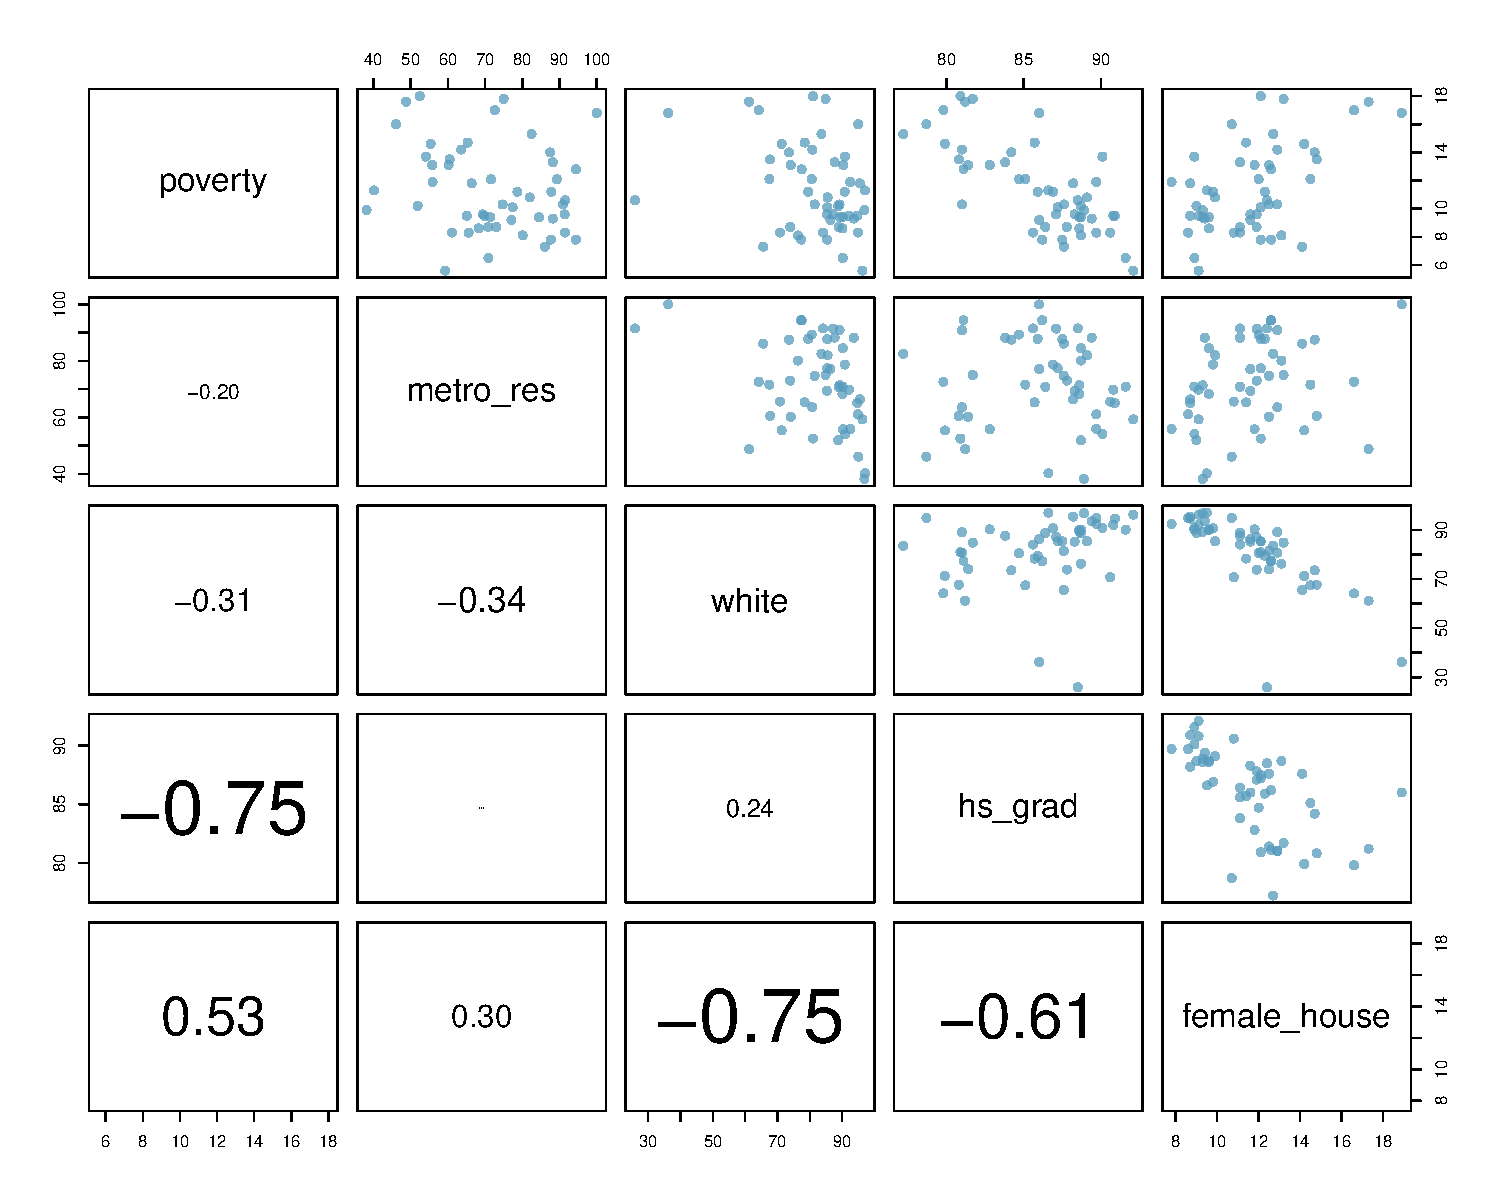
\includegraphics[width=0.98\textwidth]{figures/poverty-pairs.pdf}
\end{center}
\end{column}
\begin{column}{0.44\textwidth}
{\small The off-diagonal numbers are correlations \emph{between predictors}, not with the response.}

\vspace{0.3em}
\dq{If \texttt{white} and \texttt{female\_house} move together, what does ``holding \texttt{white} fixed'' even mean?}
\end{column}
\end{columns}

\end{frame}
%%%%%%%%%%%%%%%%%%%%%%%%%%%%%%%%%%%%%%%%%%%%%%%%%%%%%%%%%%%%%%%%%%%%%%%%
\begin{frame}
\frametitle{Collinearity inflates the standard error}

The same predictor, \texttt{female\_house}, in two models:

{\footnotesize
\begin{center}
\begin{tabular}{llrrr}
\toprule
Model & Term & Estimate & \textbf{Std. Error} & $p$-value \\
\midrule
\texttt{$\sim$ female\_house} & female\_house & 0.69 & \textbf{0.16} & 0.00 \\
\midrule
\texttt{$\sim$ female\_house} & female\_house & 0.89 & \textbf{0.24} & 0.00 \\
\texttt{\quad + white}        & white         & 0.04 & 0.04 & 0.29 \\
\bottomrule
\end{tabular}
\end{center}}

\pause
\begin{itemize}
\item The estimate \emph{moved}: $0.69 \to 0.89$.
\item The standard error \emph{inflated} by $51\%$: $0.16 \to 0.24$.
\end{itemize}

\pause
\vspace{-0.3em}
\caution{This is the signature of collinearity: the predictors carry overlapping information, so the data cannot cleanly attribute the effect to either one.}

\end{frame}
%%%%%%%%%%%%%%%%%%%%%%%%%%%%%%%%%%%%%%%%%%%%%%%%%%%%%%%%%%%%%%%%%%%%%%%%
\begin{frame}
\frametitle{Why we avoid collinear predictors}

\begin{itemize}
\item Predictors are also called \emph{independent} variables; ideally they would be independent \emph{of each other}. Collinearity breaks that.
\pause
\item Adding a predictor that duplicates one already in the model usually \hl{brings nothing new to the table}, while still costing a parameter.
\pause
\item We interpret every slope \hl{with all else held constant} --- but that phrase is not meaningful for predictors that never move separately.
\pause
\item We prefer the simplest model that does the job: a \hl{parsimonious} model.
\pause
\item Collinearity is unavoidable in observational data, but a designed \emph{experiment} can prevent it.
\vspace{-0.3em}
\end{itemize}

\end{frame}
%%%%%%%%%%%%%%%%%%%%%%%%%%%%%%%%%%%%%%%%%%%%%%%%%%%%%%%%%%%%%%%%%%%%%%%%
\begin{frame}
\frametitle{How to spot it}

\begin{columns}[T]
\column{0.5\textwidth}
\textbf{Warning signs}
\begin{itemize}
\item high correlation among predictors
\item standard errors that inflate when a predictor is added
\item a coefficient that changes a lot, or flips sign
\item large variance inflation factors (VIF)
\end{itemize}

\column{0.5\textwidth}
\textbf{VIF}
\[
\mathrm{VIF}_j = \frac{1}{1-R_j^2},
\]
where $R_j^2$ comes from predicting predictor $j$ using all the other predictors. With just two predictors, $R_j^2=r^2$. For our pair, $r=-0.751$:
\[ \frac{1}{1-0.751^2}=2.30. \]
A VIF near 1 means no overlap; large VIFs signal trouble.
\end{columns}

\end{frame}
%%%%%%%%%%%%%%%%%%%%%%%%%%%%%%%%%%%%%%%%%%%%%%%%%%%%%%%%%%%%%%%%%%%%%%%%
\section{Putting it together}
%%%%%%%%%%%%%%%%%%%%%%%%%%%%%%%%%%%%%%%%%%%%%%%%%%%%%%%%%%%%%%%%%%%%%%%%
\begin{frame}
\frametitle{Stepwise selection: a search, not a truth machine}

\begin{columns}[T]
\column{0.48\textwidth}
\textbf{Backward selection}
\begin{enumerate}
\item Start with the full model.
\item Try dropping each variable.
\item Keep the best drop.
\item Stop when no drop helps.
\end{enumerate}

\column{0.48\textwidth}
\textbf{Forward selection}
\begin{enumerate}
\item Start with the smallest model.
\item Try adding each variable.
\item Keep the best add.
\item Stop when no add helps.
\end{enumerate}
\end{columns}

\vspace{0.4em}
\caution{Stepwise search is a convenience, not a proof: it can land on different models depending on the direction and criterion, and does not replace scientific judgment.}

\end{frame}
%%%%%%%%%%%%%%%%%%%%%%%%%%%%%%%%%%%%%%%%%%%%%%%%%%%%%%%%%%%%%%%%%%%%%%%%
\begin{frame}
\frametitle{Activity: choose a model}

\activity[-- selecting a model]{%
A researcher models course evaluation score with these candidates. (\texttt{noise} is a column of random numbers.)

{\footnotesize
\begin{center}
\begin{tabular}{lcc}
\toprule
Model & Adj.\ $R^2$ & AIC \\
\midrule
M1: beauty + age & 0.071 & 720.4 \\
M2: M1 + gender & 0.083 & 714.1 \\
M3: M2 + native & 0.084 & 713.8 \\
M4: M3 + noise & 0.083 & 715.9 \\
\bottomrule
\end{tabular}
\end{center}}

Which model would you choose? What does M4 tell you?}
\end{frame}
%%%%%%%%%%%%%%%%%%%%%%%%%%%%%%%%%%%%%%%%%%%%%%%%%%%%%%%%%%%%%%%%%%%%%%%%
\begin{frame}
\frametitle{Activity: choose a model}
\solnbox{M3: highest adjusted $R^2$ \emph{and} lowest AIC, so both criteria agree. M4 is the check: a \emph{random} column made adjusted $R^2$ fall and AIC rise, so both correctly refused to pay for a useless predictor.}
\end{frame}
%%%%%%%%%%%%%%%%%%%%%%%%%%%%%%%%%%%%%%%%%%%%%%%%%%%%%%%%%%%%%%%%%%%%%%%%
\begin{frame}
\frametitle{A practical model-selection workflow}

\begin{enumerate}
\item Start from a scientific question and a sensible set of candidate predictors.
\item Fit models you could actually \emph{interpret}.
\item Compare fit against complexity: adjusted $R^2$ for linear models, AIC for any likelihood model.
\item Check for collinearity among the predictors.
\item Prefer the simplest model that answers the question well.
\item Report the uncertainty and the limitations.
\end{enumerate}

\vspace{0.4em}
A model can be statistically better yet practically worse if it is unstable, uninterpretable, or aimed at the wrong question.

\end{frame}
%%%%%%%%%%%%%%%%%%%%%%%%%%%%%%%%%%%%%%%%%%%%%%%%%%%%%%%%%%%%%%%%%%%%%%%%
\section{Wrap-up}
%%%%%%%%%%%%%%%%%%%%%%%%%%%%%%%%%%%%%%%%%%%%%%%%%%%%%%%%%%%%%%%%%%%%%%%%
\begin{frame}
\frametitle{Key takeaways}

\begin{itemize}
\item Fitting a model is easy; \emph{choosing} one is the real decision.
\item $R^2$ always rises with more predictors, so it can never select a model.
\item \hl{Adjusted $R^2$} charges for complexity, but needs a linear model.
\item \hl{AIC} $=-2\log L(\hat\theta_{MLE})+2k$ does the same job for \emph{any} likelihood model; lower is better.
\item Check for \hl{collinearity}: overlapping predictors inflate standard errors and break the ``all else held constant'' interpretation.
\item Prefer the simplest model that answers the question.
\end{itemize}

\end{frame}
%%%%%%%%%%%%%%%%%%%%%%%%%%%%%%%%%%%%%%%%%%%%%%%%%%%%%%%%%%%%%%%%%%%%%%%%

%%%%%%%%%%%%%%%%%%%%%%%%%%%%%%%%%%%%
% End document
%%%%%%%%%%%%%%%%%%%%%%%%%%%%%%%%%%%%

\end{document}
